\documentclass{article}
\usepackage{../csci-246-fall2018/hw/template/fasy-hw}
\usepackage{amsmath}
\usepackage{cancel}
\usepackage{hyperref}

\author{Nathan Stouffer}
\problem{9-1}
% \problem{A-B} means Problem Set A, Problem B.
\collab{none}
% or give names, e.g., \collab{Alyssa P. Hacker and A. Student}

\begin{document}
	
\begin{enumerate}[1.1]
	\item Find the probability such that the diagram is a four coloring. \\\\
		Let $A=\text{diagram is a four coloring}$. $P(A)=\binom{6}{4} *(\dfrac{1}{5})^4*(\dfrac{4}{5})^2=0.0153$
	\item What is the expected number of colors that will be used?
		\begin{align*}
			E(\text{number of colors})&= P(\text{1 color})*1 + P(\text{2 colors})*2 + P(\text{3 colors})*3 + P(\text{4 colors})*4 + P(\text{5 colors})*5 \\
			&= \binom{6}{1} * (\dfrac{1}{5})^6 * (\dfrac{4}{5})^0 * 1 
			+ \binom{6}{2} * (\dfrac{1}{5})^5 * (\dfrac{4}{5})^1 * 2
			+ \binom{6}{3} * (\dfrac{1}{5})^4 * (\dfrac{4}{5})^2 * 3  \\
			&+ \binom{6}{4} * (\dfrac{1}{5})^3 * (\dfrac{4}{5})^3 * 4
			+ \binom{6}{5} * (\dfrac{1}{5})^2 * (\dfrac{4}{5})^4 * 5 \\
			&= 0.000384 + 0.00768 + 0.06144 + 0.24576 + 0.49152 \\
			&= 0.806784
		\end{align*}
		Therefore, $E(\text{number of colors}) = 1$ by rounding up.
\end{enumerate}

\problem{9-2}
\collab{none}
\clearpage
\header

\section*{Section 9.1, Problem 20}

\begin{enumerate}
	\item Let $A=\text{original choice wins the prize}$. $P(A)=\dfrac{\text{winning options}}{\text{total options}}=\dfrac{1}{5}$
	\item Let $B=\text{switching doors wins the prize}$. $P(B)=\dfrac{\text{winning options}}{\text{total options}}=\dfrac{1}{4}$
\end{enumerate}

\problem{9-3}
\collab{none}
\clearpage
\header

\section*{Section 9.2, Problem 7}
a. Possibility tree
\graphicspath{ {possibility_tree} }
\begin{figure}[h]
	\centering
	\fbox{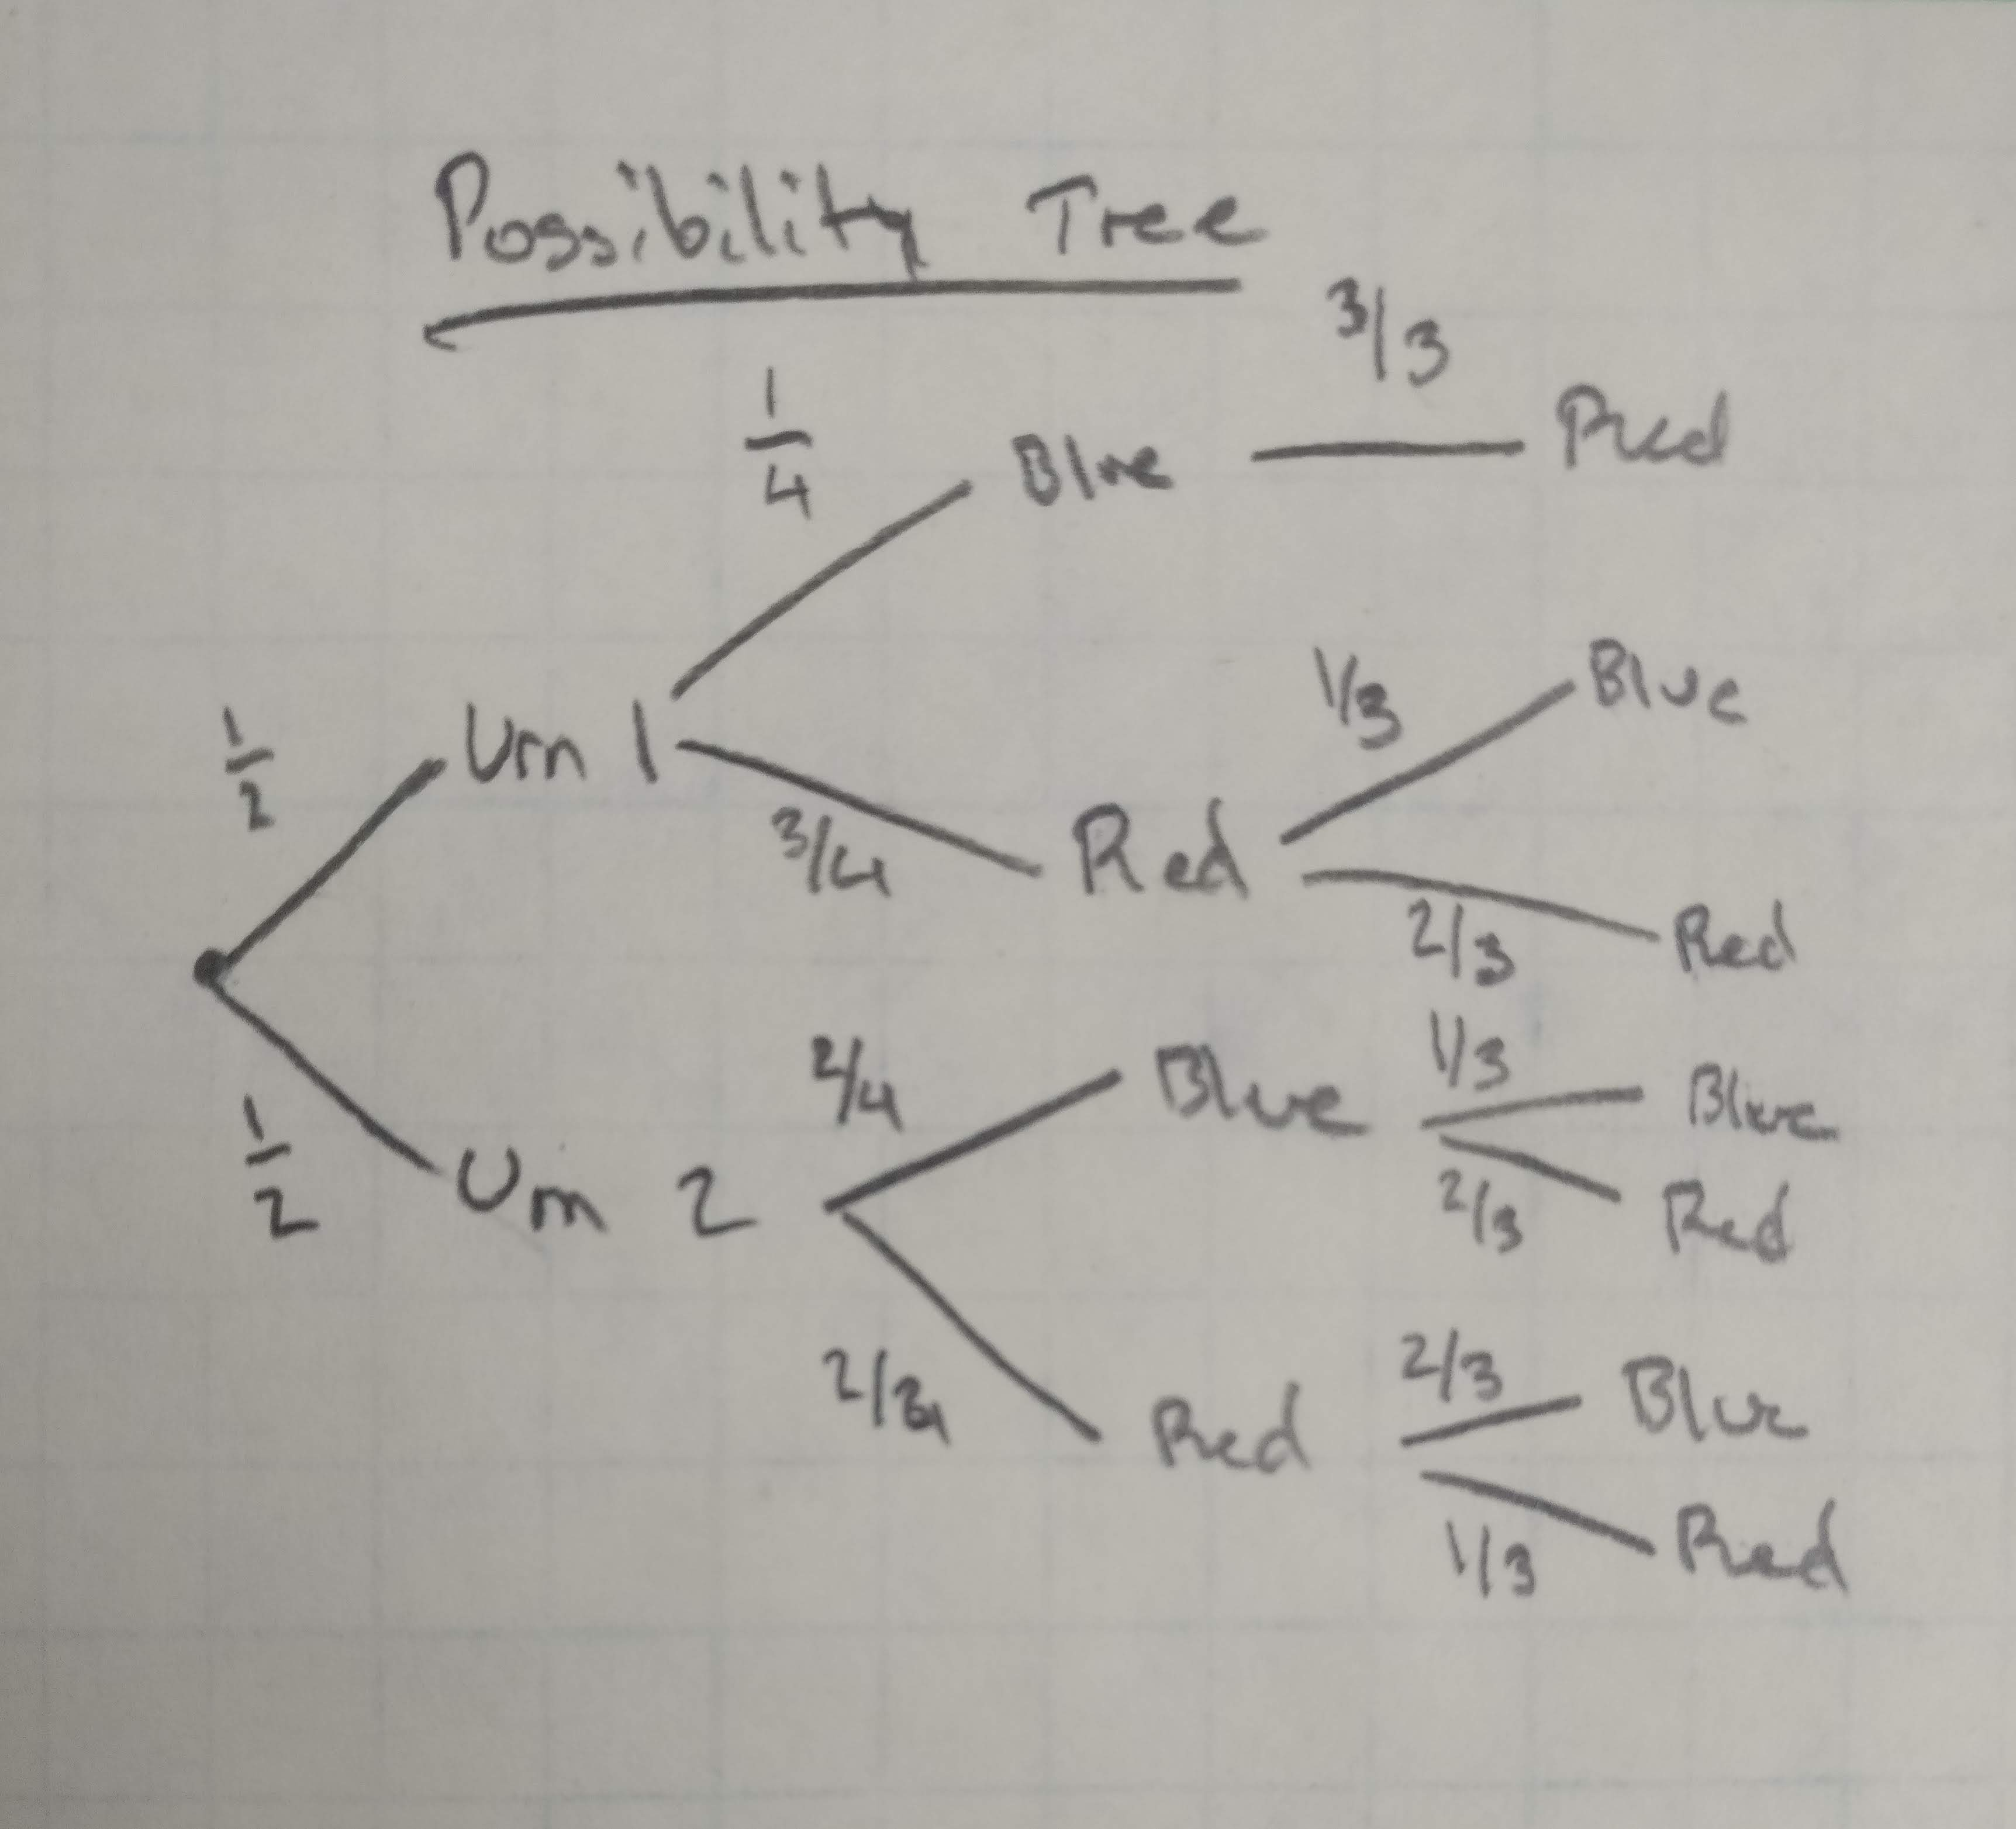
\includegraphics[width=5cm]{possibility_tree}}
	\caption{Possibility tree}
\end{figure}

b. n = number of possibliities = number of possibilites in each urn = $4*3 + 4*3=12$

c. $P(\text{2 red balls})=\dfrac{1}{2}*\dfrac{3}{4}*\dfrac{2}{3} + \dfrac{1}{2}*\dfrac{2}{4}*\dfrac{1}{3} = \dfrac{1}{4}+ \dfrac{1}{12}=\dfrac{1}{3}$

\problem{9-4}
\collab{none}
\clearpage
\header

\section*{Section 9.3, Problem 16}

\begin{enumerate}[a.]
	\item Let $p$ be the number of combinations of four hexadecimal digits without repeats. Then, $p=16*15*14*13=43680$
	\item Let $q$ be the number of combinations of four hexadecimal digits with repeats. Then, $q=(total number of combinations) - p = 16^4 - p = 21856$
	\item $P(p)=\dfrac{p}{\text{total number of combinations}}=\dfrac{21856}{16^4}=0.3335$	
\end{enumerate}

\problem{9-5}
\collab{none}
\clearpage
\header

\section*{Barbara Liskov}

References to online resources are provided as footnotes. \\

Barbara Liskov is an American Computer Scientist born in the late 1930s who made major contributions to the design of modern programming languages and is one of the most famous women in computer science. According to the Encyclopedia Britannica, Liskov also worked on "artificial intelligence projects at Stanford University."
\footnote{\url{https://www.britannica.com/biography/Barbara-Jane-Liskov}}
Liskov's contributions to programming languages make our job a lot easier in terms of design and implementation of code.

\end{document}

